\documentclass[10pt]{article}
\usepackage[margin=0.75in]{geometry}
\usepackage{graphicx,booktabs,float,caption,hyperref,microtype,amsmath}
\usepackage[T1]{fontenc}
\usepackage{lmodern}
\hypersetup{hidelinks}
\setlength{\parskip}{4pt}\setlength{\parindent}{0pt}
\title{\textbf{COP5612 Project 3 (Bonus): Failure Resilience of a Pastry Overlay in Erlang}}
\author{Surya Charan Perisetla}
\date{Fall 2026}
\begin{document}\maketitle

\section{Goal}
The base project implements the Pastry join and routing protocols (Rowstron \& Druschel) and a key/value service, with one Erlang actor per peer.
The bonus adds failures: a node can die, and a connection between two nodes can fail either temporarily or permanently.
This report describes the failure models, the mechanisms that make the overlay survive them, how resilience was tested, and what was found.

\section{Failure models}
Failures are produced by a separate \emph{injector} actor.
It schedules events at random times during the first 60\% of the request phase, which starts after every node has joined and the store has been seeded.
\begin{itemize}
  \item \textbf{Node crash} (\texttt{--kill P}): $P\%$ of the peers are killed with \texttt{exit(Pid, kill)}.
  The node gets no chance to warn anyone, and everything it stored is lost.
  \item \textbf{Temporary link failure} (\texttt{--link-temp P}): $P\%$ of the peers each pick one peer from their own routing state, and the link between the two is cut for \texttt{--link-dur} ms (3\,s by default).
  Every peer-to-peer message passes through one send function and is tagged with its sender.
  While the link is cut, both endpoints silently drop all traffic on it in both directions; the two nodes are still alive and can reach everyone else.
  \item \textbf{Permanent link failure} (\texttt{--link-perm P}): the same, but the link never recovers.
\end{itemize}

\section{Resilience mechanisms}
The mechanisms are switched on automatically whenever failures are injected, and \texttt{--no-ft} switches them off to give a baseline.
\begin{enumerate}
  \item \textbf{Per-hop acknowledgement.} Every forwarded route message carries a reference, and the receiver acknowledges it right away.
  If the ack does not arrive within 400\,ms, the sender declares the next hop failed, removes it from its leaf set, routing table and neighborhood set, and routes the message again from where it is.
  Because every Pastry hop strictly makes progress toward the key (a longer shared prefix or a numerically closer id), rerouting cannot create a loop. A 64-hop TTL is kept as a safety net and was never triggered.
  \item \textbf{Leaf-set keep-alive} (paper \S2.4). Each node pings its 16 leaves every second, and a leaf that misses two pings is declared failed.
  Each round, the node also fetches the leaf set of one random leaf, which slowly refreshes the view.
  \item \textbf{Repair} (paper \S2.4). When a leaf fails, the node asks the farthest live leaf on the same side for its leaf set and merges the answer.
  When routing-table entry $R[l][d]$ fails, the node asks another entry of row $l$ (or, if there is none, of a later row) for its own $R[l][d]$. Any such entry also has the required prefix.
  A failed peer is kept out of the tables for 10\,s, so that stale copies coming back from other nodes do not re-insert it. After that a temporarily cut link can be learned again.
  \item \textbf{Replication} (as in PAST). The root of a key stores the object and also sends it to the $K-1$ leaves closest to the key ($K=3$ by default).
  Whenever the \texttt{newLeafs} upcall reports that a node's leaf set has changed, the node sends each object it is now root of to its current replica set.
  This way the replication degree is restored after crashes.
  \item \textbf{Retries at the requester.} A request that gets no answer within 3\,s is sent again, up to 3 attempts in total.
  The retry uses the same request reference, so a late answer to the first attempt still counts.
  In the baseline the same timeout is used, but a request that times out is counted as failed.
\end{enumerate}

\section{How resilience was tested}
\textbf{Correctness oracle.} The collector actor knows every node id and which nodes have been killed.
For every answered request it checks that the node which answered is the \emph{live node numerically closest to the key}.
For a \texttt{get} of a seed object, the requester also checks that the string returned is exactly the one stored.
Each request ends in one of four outcomes:
\begin{itemize}
  \item \emph{ok}: answered with the right value;
  \item \emph{not\_found}: the request reached the root, but every copy of the object was lost;
  \item \emph{wrong\_value}: a string was returned that is not the one stored;
  \item \emph{failed}: no answer after every attempt.
\end{itemize}
In the tables below, ``correct'' means \emph{ok}.

\textbf{Experiments.} All runs use $N=1000$ peers with 10 requests each, one per second, and 3 independent seeds per configuration (96 runs).
The parameters varied were:
\begin{itemize}
  \item crash rate: 0--40\%;
  \item temporary or permanent link-failure rate: 5--40\% of the nodes;
  \item one combined scenario: 10\% crashes, 10\% temporary and 10\% permanent link failures;
  \item replication factor $K \in \{1,2,3,5\}$ at 30\% crashes.
\end{itemize}
Every configuration was run both with fault tolerance on and with \texttt{--no-ft}.
Requests whose requester was itself killed are never issued, which is why the totals drop as the crash rate rises.

\section{Results}
\begin{table}[H]
\centering\small
\caption{Node crashes ($N=1000$, $K=3$, mean of 3 runs).}
\begin{tabular}{@{}r rrr rrr@{}}
\toprule
& \multicolumn{3}{c}{\textbf{fault tolerance on}} & \multicolumn{3}{c}{\textbf{fault tolerance off}}\\
\cmidrule(lr){2-4}\cmidrule(l){5-7}
\textbf{crashed} & correct & object lost & avg hops & correct & no answer & avg hops\\
\midrule
0\%  & 100.00\% & 0.00\% & 2.48 & 100.00\% & 0.00\% & 2.48\\
5\%  & 100.00\% & 0.00\% & 2.50 & 92.53\% & 7.47\% & 2.47\\
10\% & 99.99\% & 0.01\% & 2.51 & 85.86\% & 14.14\% & 2.46\\
20\% & 99.87\% & 0.13\% & 2.55 & 74.22\% & 25.78\% & 2.43\\
30\% & 99.78\% & 0.22\% & 2.57 & 66.32\% & 33.68\% & 2.43\\
40\% & 99.28\% & 0.72\% & 2.58 & 60.40\% & 39.60\% & 2.41\\
\bottomrule
\end{tabular}
\end{table}

\begin{table}[H]
\centering\small
\caption{Link failures ($N=1000$, $K=3$, mean of 3 runs): share of requests answered correctly.}
\begin{tabular}{@{}r rr rr@{}}
\toprule
& \multicolumn{2}{c}{\textbf{temporary (3 s)}} & \multicolumn{2}{c}{\textbf{permanent}}\\
\cmidrule(lr){2-3}\cmidrule(l){4-5}
\textbf{nodes with a cut link} & FT on & FT off & FT on & FT off\\
\midrule
5\%  & 100.00\% & 99.85\% & 100.00\% & 99.67\%\\
10\% & 100.00\% & 99.66\% & 99.99\% & 99.37\%\\
20\% & 100.00\% & 99.44\% & 99.96\% & 98.76\%\\
40\% & 100.00\% & 98.85\% & 99.94\% & 97.52\%\\
\midrule
\multicolumn{5}{@{}l}{Combined 10\% crash + 10\% temp + 10\% perm: FT on 99.99\%, FT off 85.66\%.}\\
\bottomrule
\end{tabular}
\end{table}

\begin{figure}[H]
\centering
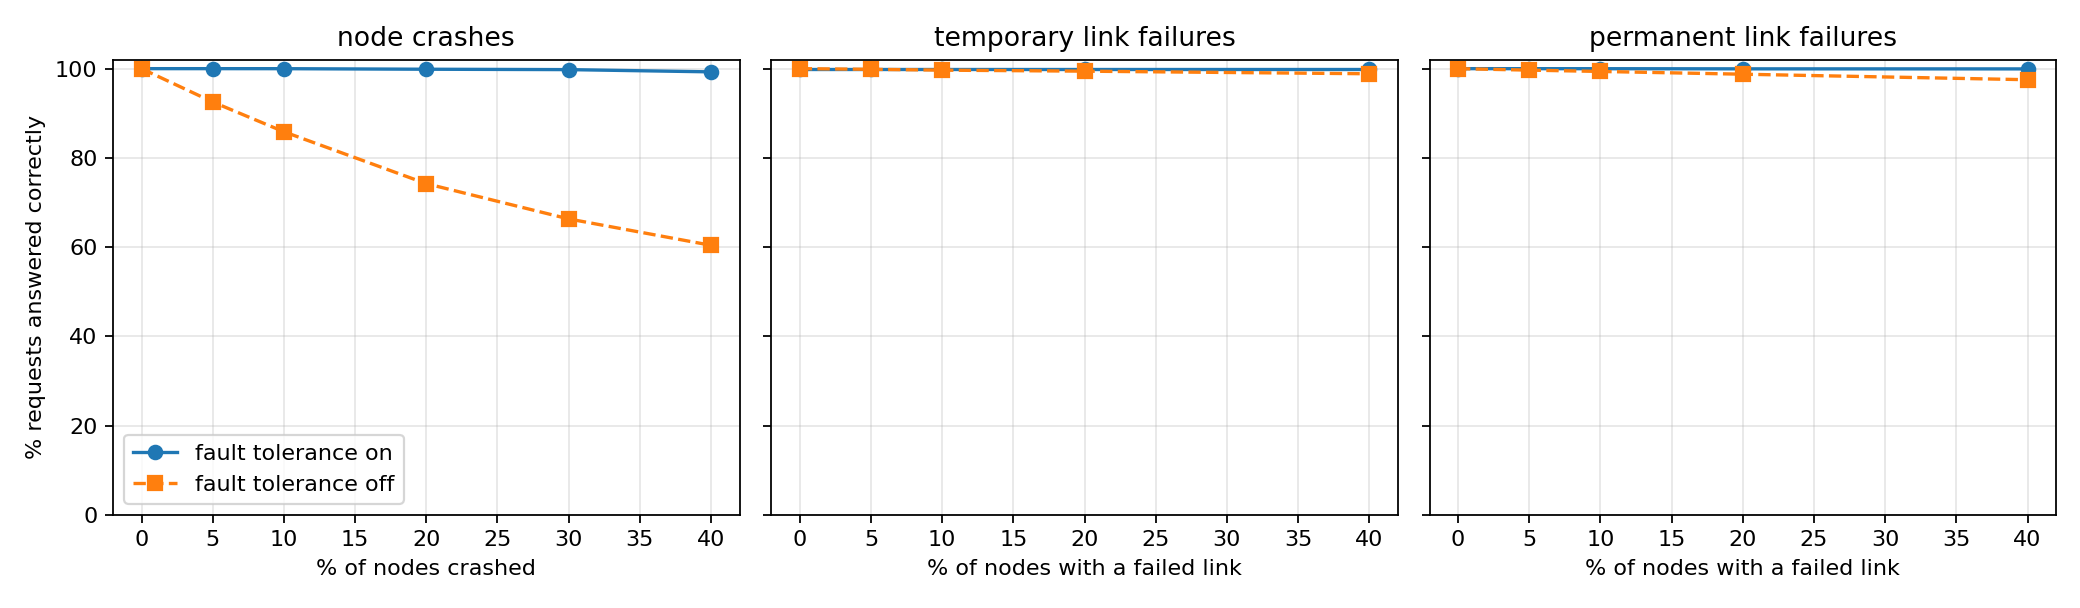
\includegraphics[width=\linewidth]{bonus_success.png}
\caption{Share of requests answered correctly, with fault tolerance on and off.}
\end{figure}

\begin{figure}[H]
\centering
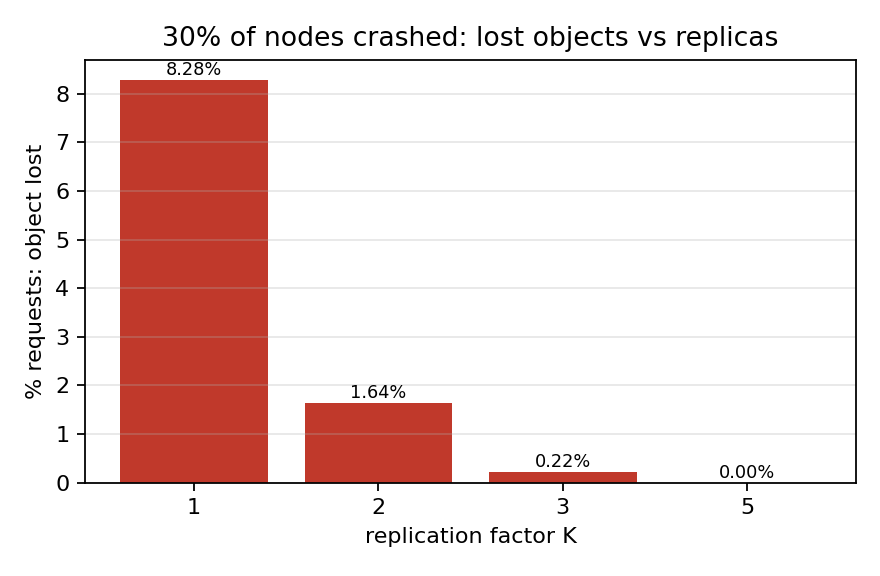
\includegraphics[width=0.55\linewidth]{bonus_replicas.png}
\caption{Share of requests that found their object lost at 30\% crashes, versus the replication factor $K$ (all with fault tolerance on).
$K=1$: 8.28\%, $K=2$: 1.64\%, $K=3$: 0.22\%, $K=5$: 0\%.}
\end{figure}

\section{Findings}
\begin{itemize}
  \item \textbf{Routing survives crashes.} With fault tolerance on, not one request was left unanswered in any crash experiment, even with 40\% of the nodes killed.
  Every answered request also reached the live node closest to the key (at most one exception per run).
  Without fault tolerance, roughly every crashed node in the path loses the message, so the loss grows with the crash rate, reaching 40\% unanswered at 40\% crashes.
  \item \textbf{Routing costs little extra.} The average path grows only from 2.48 to 2.58 hops at 40\% crashes.
  A failed hop costs one 400\,ms timeout and one reroute, and repairs keep the tables close to optimal.
  (The baseline hop count is slightly \emph{lower} only because it is averaged over the messages that survived.)
  \item \textbf{Replication is what keeps the data.} Routing alone cannot help if every copy of an object is gone.
  With $K=1$ and 30\% crashes, 8.3\% of reads found their object lost.
  Replication plus re-replication on \texttt{newLeafs} reduces this to 1.6\% ($K=2$), 0.22\% ($K=3$) and 0\% ($K=5$).
  The losses that remain occur when all $K$ copies die before the leaf sets have been repaired.
  \item \textbf{Link failures are mild but still matter.} Only one hop is affected, so even the baseline loses just 1--2.5\% of requests at 40\%.
  With fault tolerance on, temporary failures never caused a lost request, and permanent ones caused at most 0.06\%.
  A cut link does lead to a few ``misrouted'' answers (up to 29 per 10\,000 requests in a single run): a node whose only link to its true ring neighbour is cut cannot see that neighbour, so it answers for that neighbour's keys itself.
  This is the expected behaviour of a partially partitioned overlay. Because both nodes are still alive and hold replicas, the value returned was still correct in every case (zero \emph{wrong\_value}).
  \item \textbf{Cost.} The keep-alives add 16 pings and one leaf-set exchange per node per second, and the per-hop acks double the routing traffic.
  This overhead is why fault tolerance is enabled only when failures are injected. The failure-free results of the main project are measured without it.
\end{itemize}

\section{Reproducing}
A single run looks like this: \texttt{./project3 1000 10 --kill 30 --link-temp 10 --replicas 3}.
\end{document}
